
\documentclass[12pt]{article}
\usepackage[a4paper]{geometry}
\usepackage{natbib}
% Necessary packages
\usepackage[english]{babel}
\usepackage[utf8]{inputenc}
\usepackage[T1]{fontenc}
\usepackage{lmodern}
\usepackage{graphicx}
\usepackage{amsmath, amssymb}
\usepackage{geometry}
\usepackage{fancyhdr}
\usepackage{setspace}
\usepackage{hyperref}
%\usepackage[font={bf}]{caption}
\usepackage{subcaption} % Package pour les sous-figures
\usepackage{float}
\usepackage[section]{placeins}
\usepackage[colorlinks=true, allcolors=blue]{hyperref}


@article{jaravel2023politiques,
  title={Les politiques publiques au défi du retour de l’inflation},
  author={Jaravel, X. and Méjean, I. and Ragot, X.},
  journal={Notes du conseil d'analyse économique},
  volume={78},
  pages={1-12},
  year={2023},
  doi={10.3917/ncae.078.0001}
}



\subsection{Inflation Inequalities Developments}
\label{sec:analyse-donnees}


%%%%%%%%%%%%%%%%%%%%%%%%%%%%%%%%%%%%%%%%%%%%%%%%%%%%%%%%%%%%%%
\begin{figure}[!ht]
\centering
\caption{Inflation by Income Quintile (first quintile, fifth quintile)  (in \%)
\label{fig:italy_spain}
}
\begin{subfigure}{0.48\textwidth} 
  \centering
  \caption{Italy}
  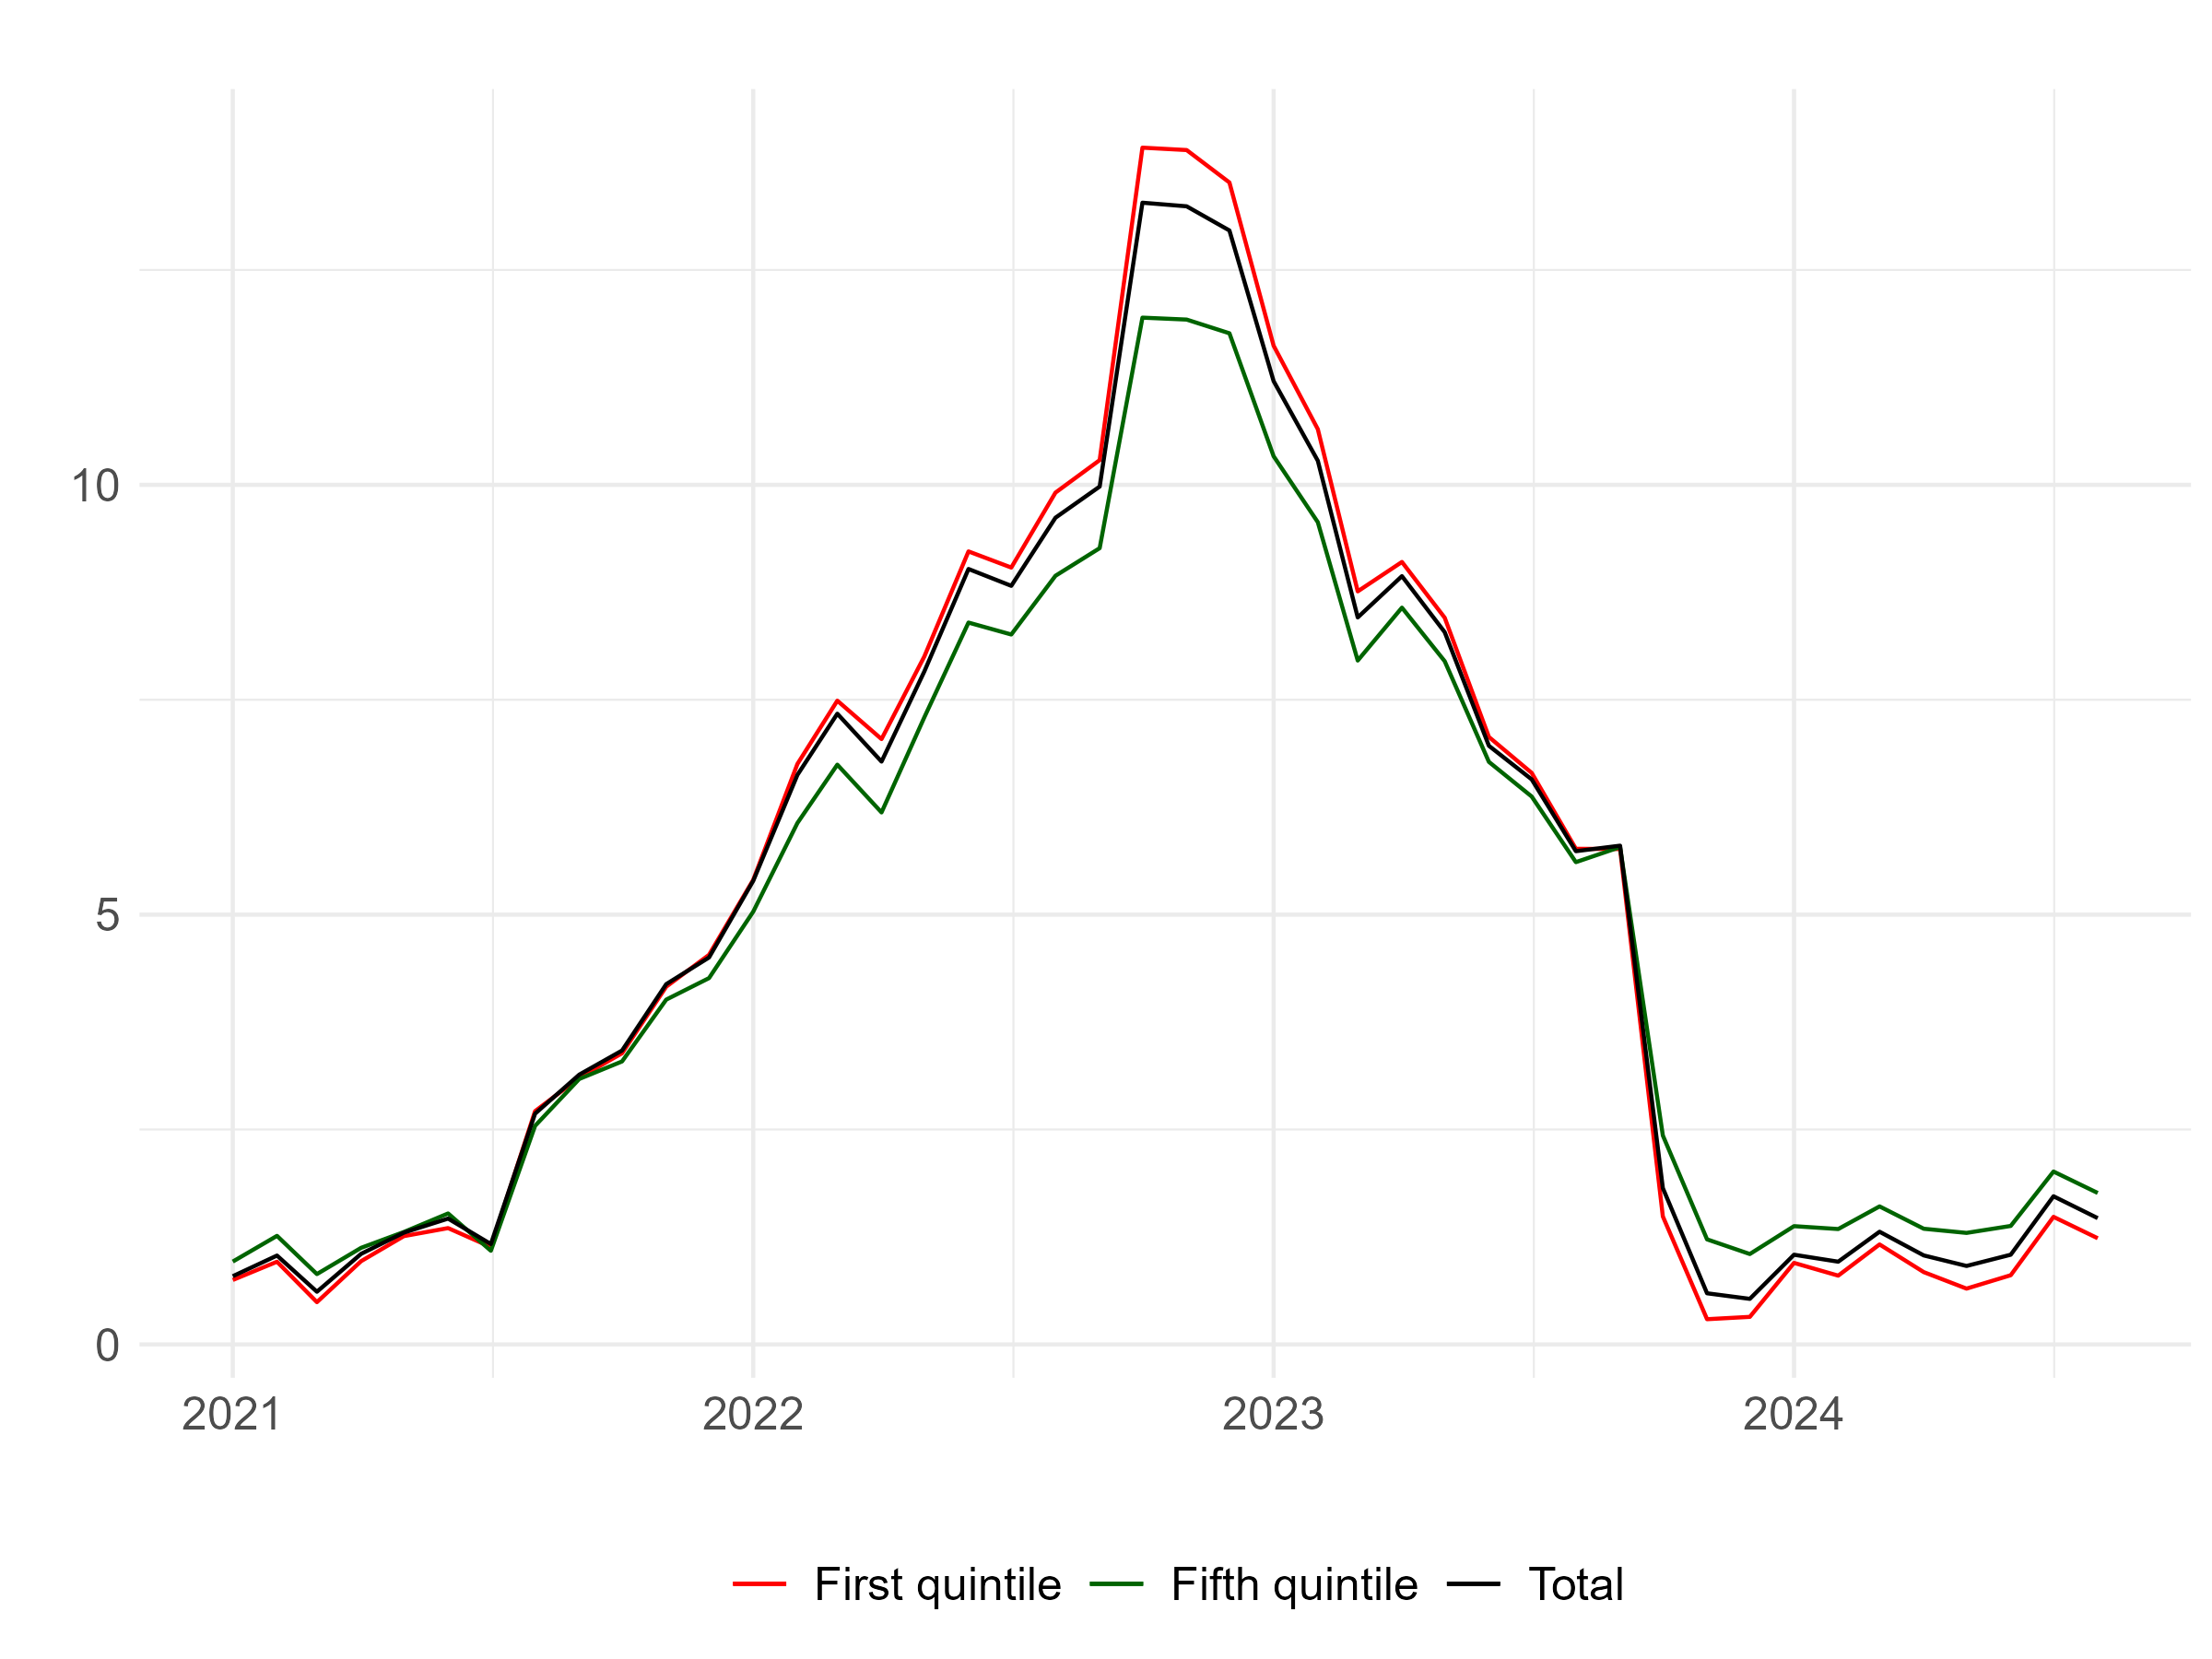
\includegraphics[width=\linewidth,height=6cm]{fig/figure8.png}
\end{subfigure}
\hfill 
\begin{subfigure}{0.48\textwidth} 
  \centering
  \caption{Spain}
  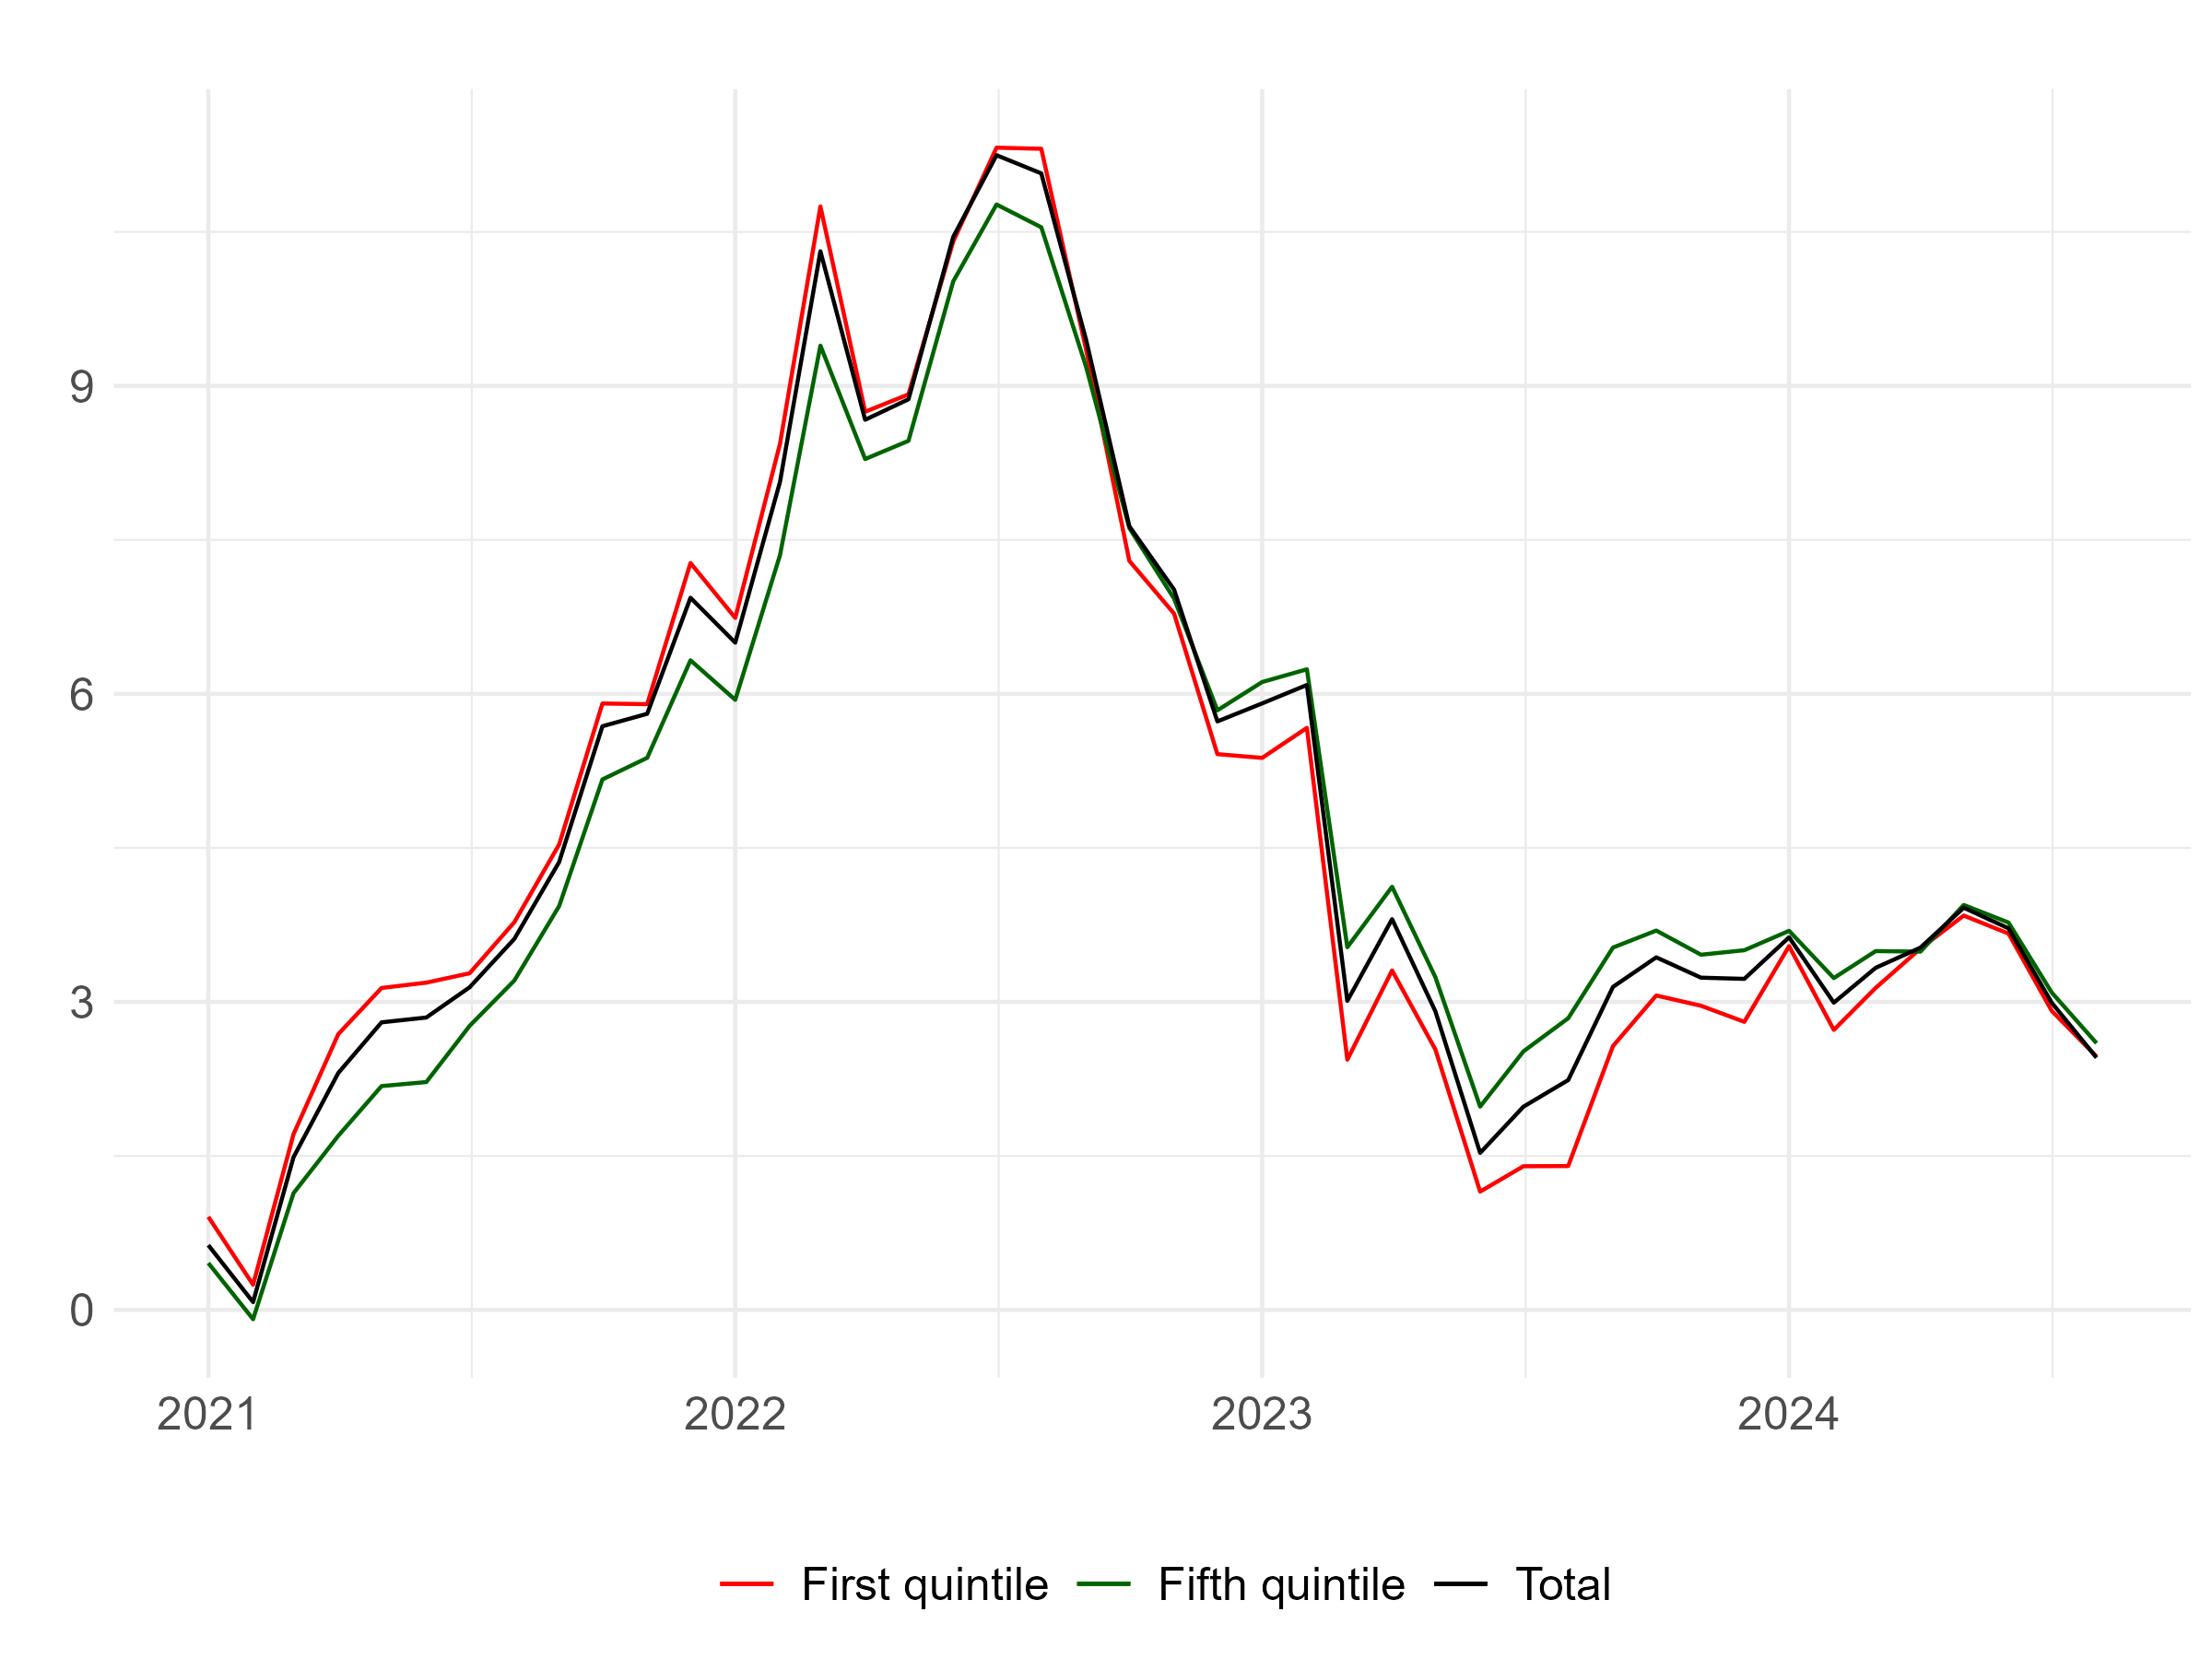
\includegraphics[width=\linewidth,height=6cm]{fig/figure9.png}
\end{subfigure}
%\label{fig:dev}
\vspace{10pt} 
\captionsetup{font=footnotesize, format=hang, singlelinecheck=false, justification=justified}
\caption*{Note:.\\
Sources: Eurostat, authors' calculation}
\label{sec:analyse-donnees}
\end{figure}
%%%%%%%%%%%%%%%%%%%%%%%%%%%%%%%%%%%%%%%%%%%%%%%%%%%%%%%%%%%%%%
\newpage

The contrasting experiences of Italy and Spain highlight how country-specific factors, including both economic structure and policy responses, shaped inflation inequality outcomes. Italy's wider inflation differentials reflect both its higher energy dependency and more limited deployment of price shield measures, while Spain's more moderate differentials suggest its price control policies were relatively effective at containing distributional impacts.

Figure 4 illustrates the inflation rates experienced by the first and fifth income quintiles.


%Several recent contributions have re-evaluated the heterogeneity of inflation linked to differences in consumption structure between households, in conjunction with the new availability of granular data (individual survey, cash register and bank customer data). These data make it possible to calculate inflation directly at household level, rather than by household category. Jaravel (2021) finds a higher level of inequality with cash register data than with data from the Consumer Expenditure Survey in the USA during a period of low inflation between 2004 and 2015. Indeed, with the standard approach, he obtains an inflation gap of 0.37 pp. 

%On the other hand, on a comparable field using cash data, he finds an inflation gap of 0.66 pp (i.e. first quintile inflation of 1.87\% and last quintile inflation of 1.21\%). Menuyert (2022) has carried out a similar exercise for all European Union countries. 

%Bank customer data can be used to estimate the effects of consumption, income and wealth simultaneously (Cardoso et al., 2022, Pallotti et al. 2023), using general equilibrium modeling. Thus, Cardoso et al. (2022) show that the distributional effect of inflation passing through household wealth and income is greater than that of consumption in Spain. In a similar vein, Palloti et al (2023) also find that net household wealth is the key factor in inequality in the face of inflation in the six euro area countries (Germany, France, Italy, Spain, the Netherlands and Belgium). They separate the direct effect of inflation on households from the general equilibrium effects via wages, rents and asset prices. They find that the direct effect is greater than the general equilibrium effects. Overall, income losses are of the order of 6\% as a result of the 2021-23 inflationary episode. Older households are by far the ones to lose out as a result of the effect on wealth. 


%Bank client data offers high-frequency insights into consumption and income, enabling a more comprehensive analysis of both inflation exposure and experiences.



%%%%%%%%%%%%%%%%%%%%%%%%%%%%%%%%%%%%%%%%%%%%%%%%%%%%%%%%%%%%%%
\begin{figure}[!ht]
\centering
\caption{Comparison with Harmonized CPI in Spain (inflation in \%, offset in pp)}
%\label{fig:Fig4.png}
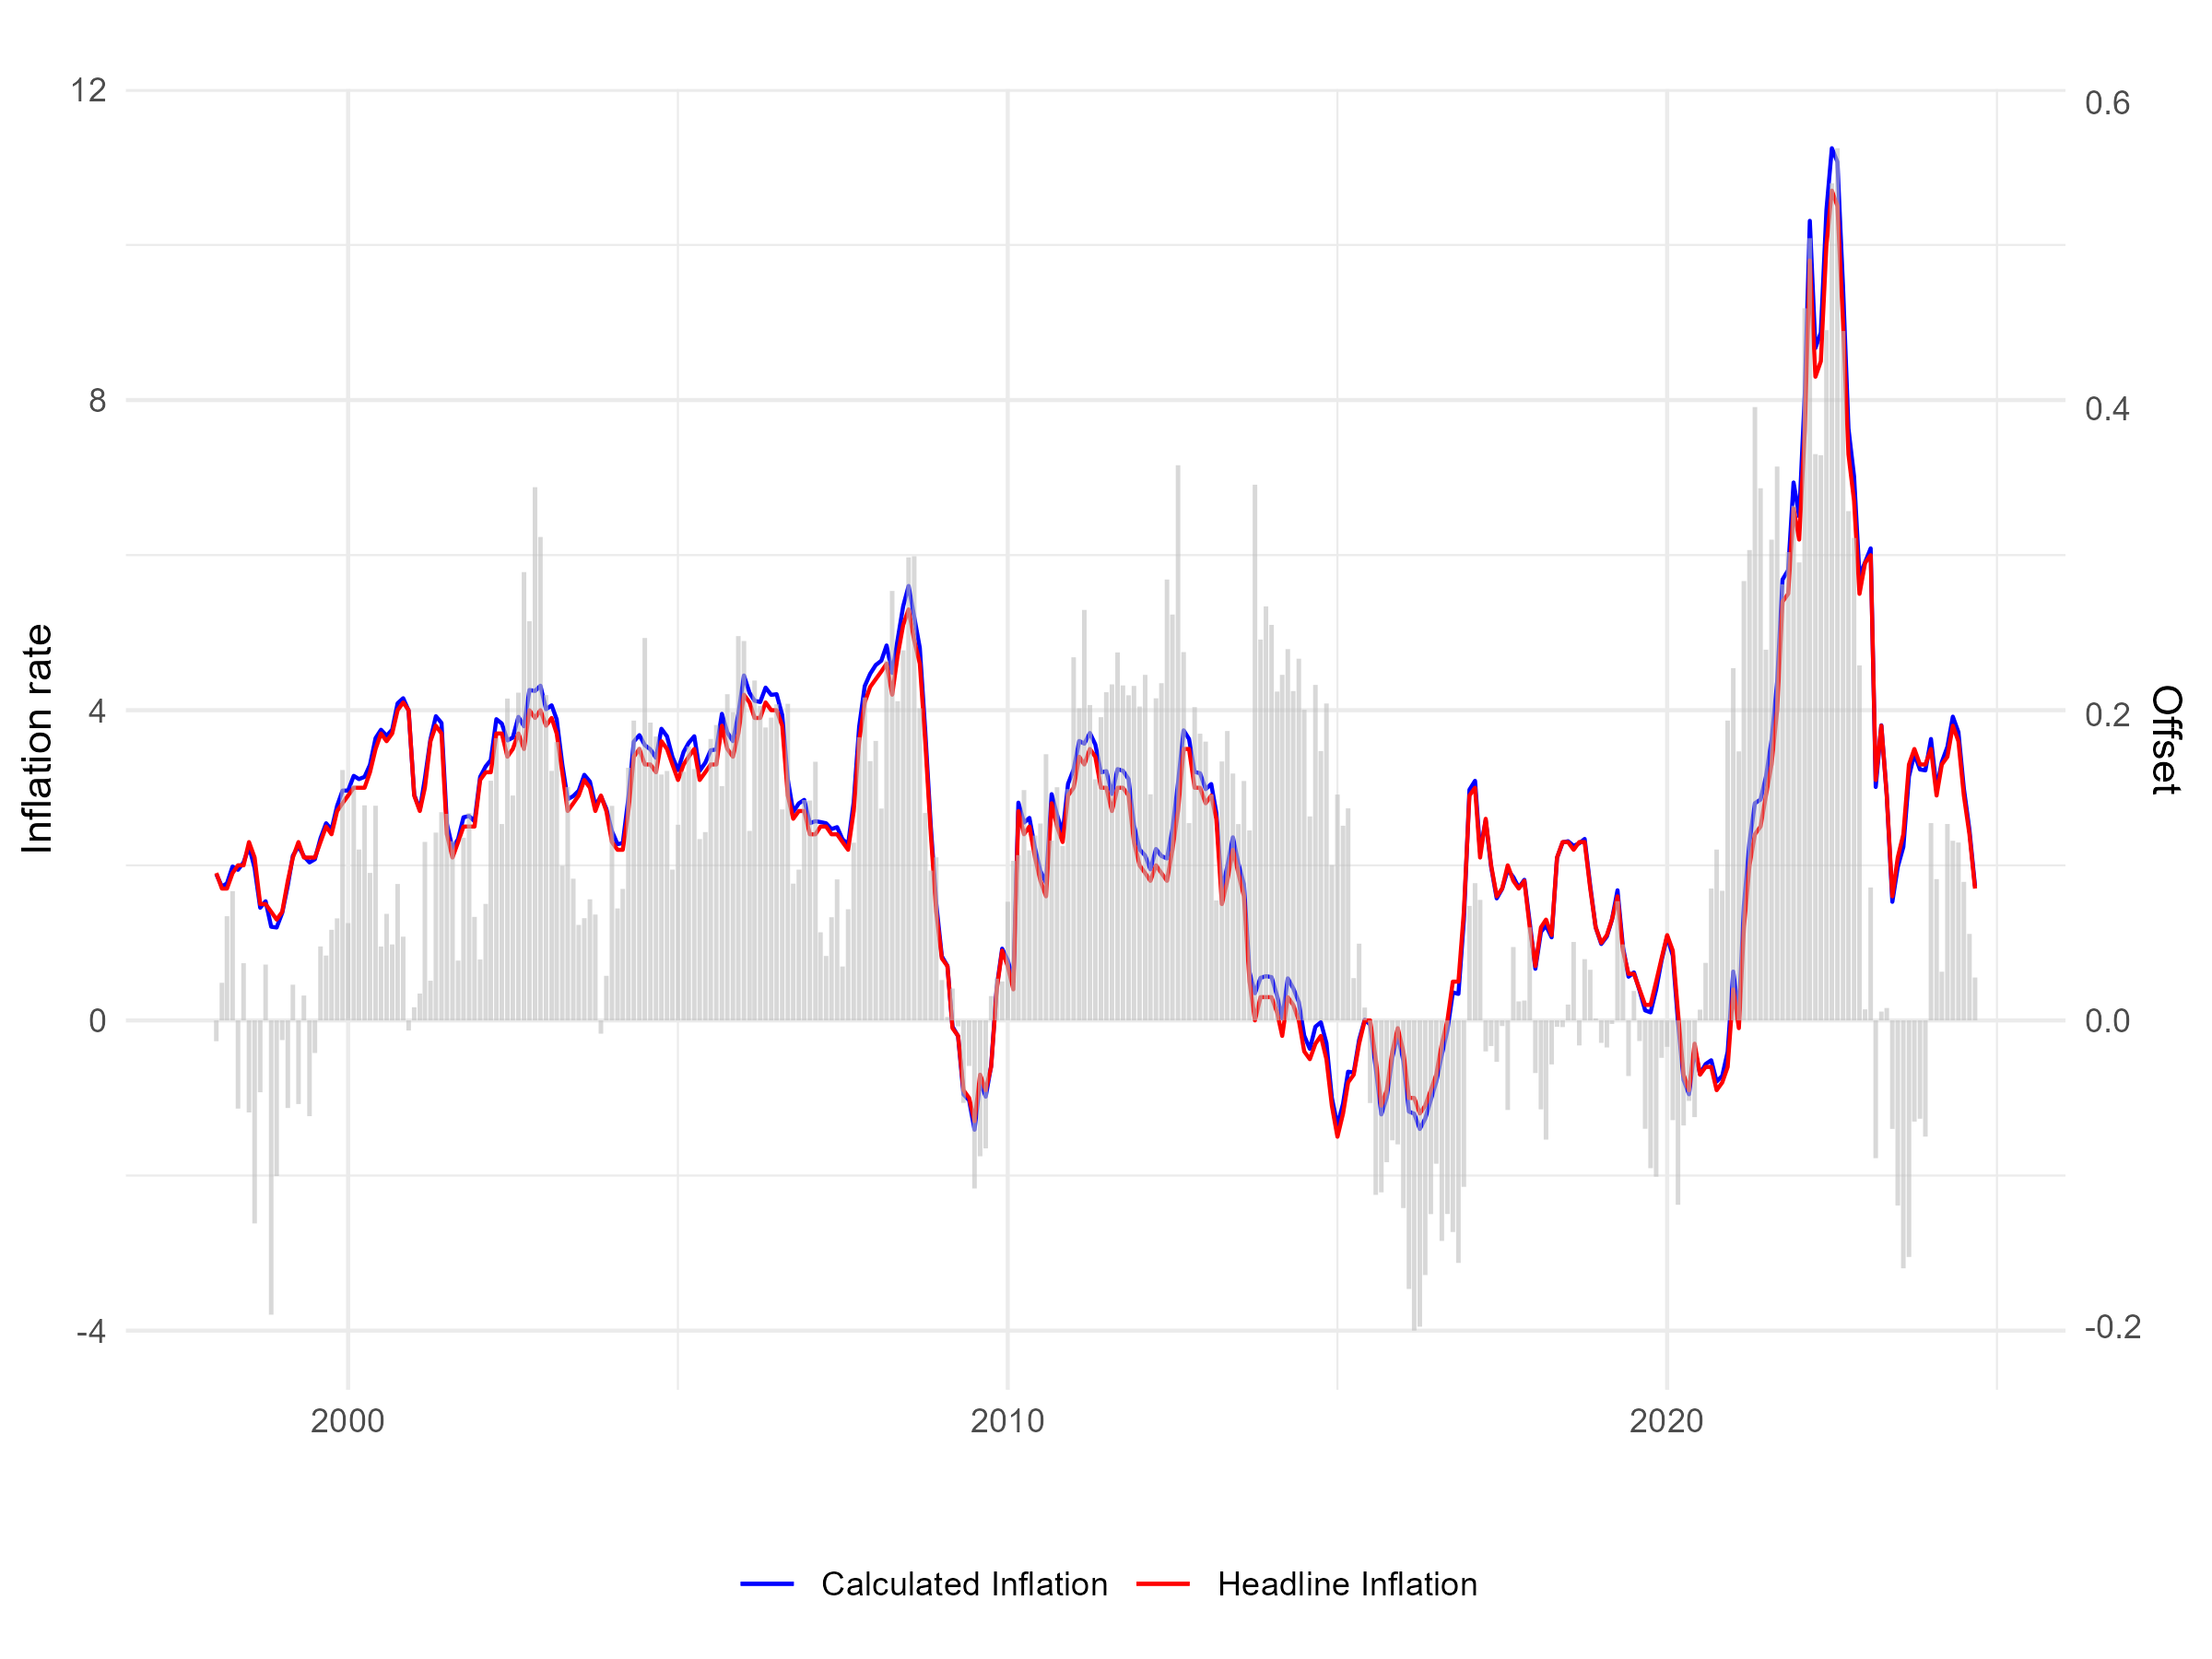
\includegraphics[scale=0.7]{fig/figureA.PNG}
\vspace{20pt} 
\captionsetup{font=footnotesize, format=hang, singlelinecheck=false, justification=justified}
\caption*{Note: This figure compares the inflation published by Eurostat to the inflation built using publicly-available data.
Sources: Eurostat, authors' calculation}
\end{figure}
%%%%%%%%%%%%%%%%%%%%%%%%%%%%%%%%%%%%%%%%%%%%%%%%%%%%%%%%%%%%%%

